%!TEX root = ../BUSystematics.tex

\graphicspath{{Body/Figures/Gain/IFG/60h/Amplitude/}{Body/Figures/Gain/IFG/60h/Amplitude-With-AdHoc/}{Body/Figures/Gain/IFG/60h/Lifetime/}{Body/Figures/Gain/IFG/9d/Lifetime/}{Body/Figures/Gain/ResidualGain/EnergyBinKloss/}{Body/Figures/Gain/ResidualGain/Chi2Min/}}

\section{Gain Systematic Errors}



-Describe generalities of gain effects here






\begin{table}
\centering
\setlength\tabcolsep{10pt}
\renewcommand{\arraystretch}{1.2}
\begin{tabular*}{1\linewidth}{@{\extracolsep{\fill}}lHHHH}
  \hline
    \multicolumn{5}{c}{\textbf{Gain Correction Parameter Errors}} \\
  \hline
    Quantity & \thead{60h} & \thead{HighKick} & \thead{9d} & \thead{Endgame} \\
  \hline
    IFG Amplitude      & 21.4 & 6.3 & 15.3  & 3.7 \\
    IFG Time Constant  & 16.1 & 6.5 & 11.5 & 6.5 \\
    STDP Amplitude     & 1.9 & 1.9 & 1.9 & 1.9 \\
    STDP Time Constant & 3.4  & 3.4 & 3.4 & 3.4 \\
  \hline 
\end{tabular*}
\caption[]{Average uncertainties on the crystal gain correction parameters, weighted by the number of counts put into the T-Method histogram, as determined by D. Sweigart, left side of Table 6.5 \cite{phdthesis:2020Sweigart} for 60h and 9d datasets, and personal communication/spreadsheet for the HK and EG datasets \cite{UncertaintySpreadsheet} (which used the tau ltdp). Original data can be found in \cite{GainElog1,GainElog2,GainElog3,GainElog4}. All STDP parameters were the same as calculated from the same STDP laser data. The author calculated the average (not hit-weighted) uncertainties, and found less than a percent difference in each case. Units are in percent.}
\label{tab:gainCorrErrs}
\end{table}




% Keep in mind that for HighKick and Endgame the crystal gain lifetime parameters were fixed to tau_ltdp, using the same study. 

% For HighKick and Endgame the corrections go as STDP, OOF, IFG. 
% For 60h and 9d the corrections go as OOF, STDP, IFG.

% HighKick had some steps in the CTAGs.





% - need to compare R vs T method results
% - need to reference the errors used for the amplitude and the lifetime - hit weighted numbers David came up with for some datasets, and standard errors for the other datasets with the fixed tau ltdp
% -record those errors into my table so people know exactly what they are
% - describe the reasoning for the range for the linear fit in the lifetime case - perhaps include figures from other datasets showing the behavior
% - point out that these two errors are highly correlated but I'm being very conservative and adding them in quadrature
% - mention STDP as the results from with vs without the effect - reiterate that with my randomization scheme I don't have to worry about the statistics part as much, briefly mention that I don't have the ability to scan over the effect since I do things at the histogram level - do mention that I use Aaron's gain corrector module to make the trees...
% - decide what I want to do for the ad hoc gain scan and then explain those results, include relevant plots, include updated plots for the IFG scan showing consistency with 1 afteer I have done so





\subsection{IFG Amplitude}


The systematic error due to the IFG amplitude was determined by 




\begin{figure}[h]
\centering
    \begin{subfigure}[t]{0.45\textwidth}
        \centering
        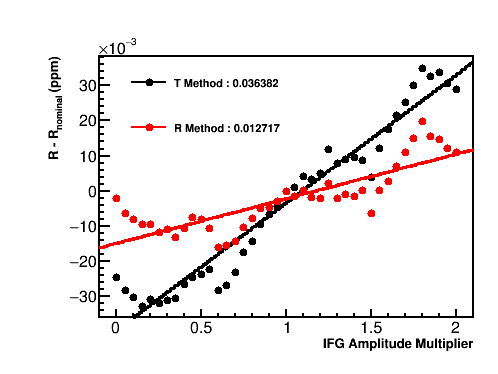
\includegraphics[width=\textwidth]{IFG_Amplitude_Compare_R}
        \caption{}
    \end{subfigure}% %you need this % here to add spacing between subfigures
    \hspace{1cm}
    \begin{subfigure}[t]{0.45\textwidth}
        \centering
        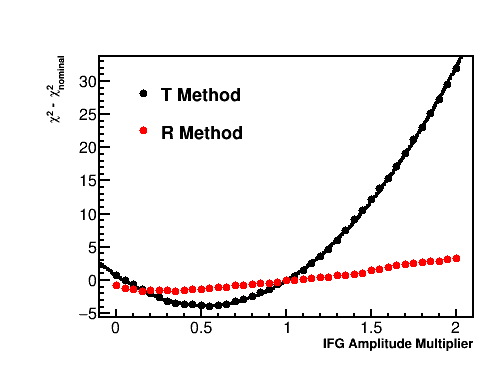
\includegraphics[width=\textwidth]{IFG_Amplitude_Compare_Chisq.png}
        \caption{}
    \end{subfigure}
\caption[Systematic error due to]{Systematic error due to. Data are from the 60h dataset.}
\label{fig:IFGAmpscan}
\end{figure}





\begin{table}[h]
\centering
% \setlength\tabcolsep{10pt}
\renewcommand{\arraystretch}{1.2}
\begin{tabularx}{0.9\linewidth}{XOOJ}
  \hline
    \multicolumn{4}{c}{\textbf{IFG Amplitude Scan Results}} \\
  \hline\hline
    Dataset & \thead{Fit Method} & \multicolumn{1}{c}{$dR/dA_{ifg}$} & \multicolumn{1}{c}{$\boldsymbol{\delta R}$} \\
  \hline
    \multirow{2}{*}{60h} & T & 36.4 & 7.8 \\
                         & R & 12.7 & 2.7 \\
  \hline
    \multirow{2}{*}{HighKick} & T & 52.1 & 3.3 \\
                              & R & 8.4 & 0.5 \\
  \hline
    \multirow{2}{*}{9d} & T & 29.6 & 4.5 \\
                        & R & 9.7 & 1.5 \\
  \hline
    \multirow{2}{*}{Endgame} & T & 64.0 & 2.4 \\
                             & R & 27.9 & 1.0 \\
  \hline
\end{tabularx}
\caption[]{}
\label{tab:IFGampScan}
\end{table}






\subsection{IFG Time Constant}


- range from 0.8 to 1.5, determined from inspection of the various datasets, and then made the same for all datasets.


\begin{figure}[h]
\centering
    \begin{subfigure}[t]{0.45\textwidth}
        \centering
        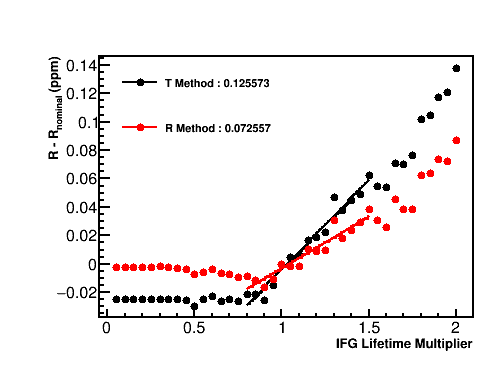
\includegraphics[width=\textwidth]{IFG_Lifetime_Compare_R}
        \caption{}
    \end{subfigure}% %you need this % here to add spacing between subfigures
    \hspace{1cm}
    \begin{subfigure}[t]{0.45\textwidth}
        \centering
        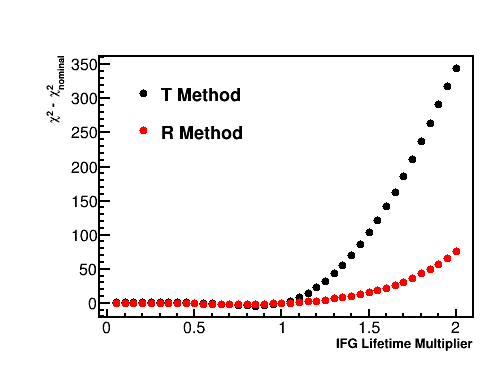
\includegraphics[width=\textwidth]{IFG_Lifetime_Compare_Chisq}
        \caption{}
    \end{subfigure}
\caption[Systematic error due to]{Systematic error due to. Data are from the 60h dataset.}
\label{fig:IFGAmpscan}
\end{figure}


\begin{figure}[h]
\centering
    \begin{subfigure}[t]{0.45\textwidth}
        \centering
        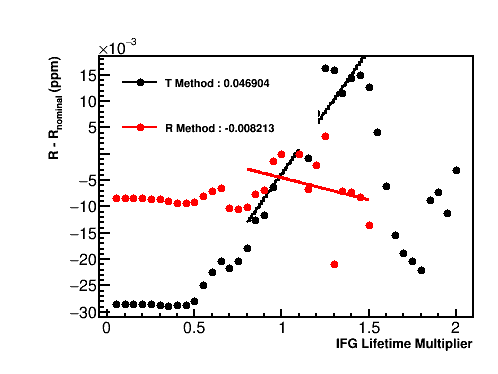
\includegraphics[width=\textwidth]{IFG_Lifetime_Compare_R_9d}
        \caption{}
    \end{subfigure}% %you need this % here to add spacing between subfigures
    \hspace{1cm}
    \begin{subfigure}[t]{0.45\textwidth}
        \centering
        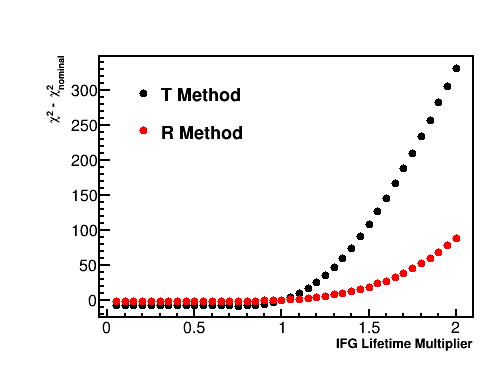
\includegraphics[width=\textwidth]{IFG_Lifetime_Compare_Chisq_9d}
        \caption{}
    \end{subfigure}
\caption[]{Systematic error due to. Data are from the 9d dataset.}
\label{fig:IFGAmpscan}
\end{figure}


- should I include the awkward looking 9d plot here?




\begin{table}[h]
\centering
% \setlength\tabcolsep{10pt}
\renewcommand{\arraystretch}{1.2}
\begin{tabularx}{0.9\linewidth}{XOOK}
  \hline
    \multicolumn{4}{c}{\textbf{IFG Time Constant Scan Results}} \\
  \hline\hline
    Dataset & \thead{Fit Method} & \multicolumn{1}{c}{$dR/d\tau_{ifg}$} & \multicolumn{1}{c}{$\boldsymbol{\delta R}$} \\
  \hline
    \multirow{2}{*}{60h} & T & 125.6 & 20.2 \\
                         & R & 72.6 & 11.7 \\
  \hline
    \multirow{2}{*}{HighKick} & T & 150.4 & 9.8 \\
                              & R & 49.7 & 3.2 \\
  \hline
    \multirow{2}{*}{9d} & T & 46.9 & 5.4 \\
                        & R & 8.2 & 0.9 \\
  \hline
    \multirow{2}{*}{Endgame} & T & 204.5 & 13.3 \\
                             & R & 101.3 & 6.6 \\
  \hline
\end{tabularx}
\caption[]{}
\label{tab:IFGtauScan}
\end{table}






\subsection{STDP}


- turned it on and off 





\begin{table}[h]
\centering
% \setlength\tabcolsep{10pt}
\renewcommand{\arraystretch}{1.2}
\begin{tabularx}{0.9\linewidth}{XOOK}
  \hline
    \multicolumn{4}{c}{\textbf{STDP Results}} \\
  \hline\hline
    Dataset & \thead{Fit Method} & \multicolumn{1}{c}{$\Delta R_{\text{(w/ - w/o)}}$} & \multicolumn{1}{c}{$\boldsymbol{\delta R}$} \\
  \hline
    \multirow{2}{*}{60h} & T & 4.8 & 0.1 \\
                         & R & 2.8 & 0.1 \\
  \hline
    \multirow{2}{*}{HighKick} & T & 2.2 & 0.1 \\
                              & R & 2.2 & 0.1 \\
  \hline
    \multirow{2}{*}{9d} & T & 11.2 & 0.2 \\
                        & R & 14.0 & 0.3 \\
  \hline
    \multirow{2}{*}{Endgame} & T & 3.9 & 0.1 \\
                             & R & 5.0 & 0.1 \\
  \hline
\end{tabularx}
\caption[]{}
\label{tab:systematicError_STDP}
\end{table}








\subsection{Residual Gain Variation}


% -potentially talk about both ways to get the value for the amplitdue, chi2 min and flatten k_loss - and show plots for this
% -give equation for residual gain and show which values I used, and then cite Aaron's work for the value I used
% did energy bin fits with T method, only main CBO parameters, applied various ad hoc gain amplitudes to try and flatten out the spectrum


\begin{figure}[h]
\centering
    \begin{subfigure}[t]{0.45\textwidth}
        \centering
        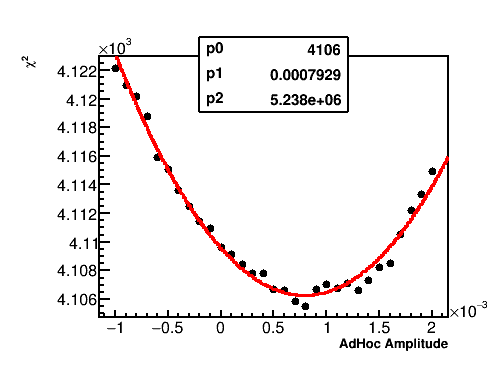
\includegraphics[width=\textwidth]{TMethod_Chi2_Vs_AdHocAmplitude_Canv}
        \caption{T-Method \chisq versus pileup multiplier. The parabolic fit equation used was $y = p_{2}(x - p_{1})^{2} + p_{0}.$}
    \end{subfigure}% %you need this % here to add spacing between subfigures
    \hspace{1cm}
    \begin{subfigure}[t]{0.45\textwidth}
        \centering
        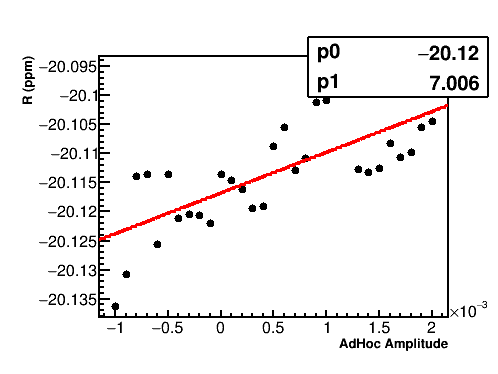
\includegraphics[width=\textwidth]{TMethod_R_Vs_AdHocAmplitude_Canv}
        \caption{T-Method $R$ versus pileup multiplier. The parameter $p_{1}$ gives the sensitivity of $R$ to the value of the pileup multiplier, with units in ppm.}
    \end{subfigure}

    \begin{subfigure}[t]{0.45\textwidth}
        \centering
        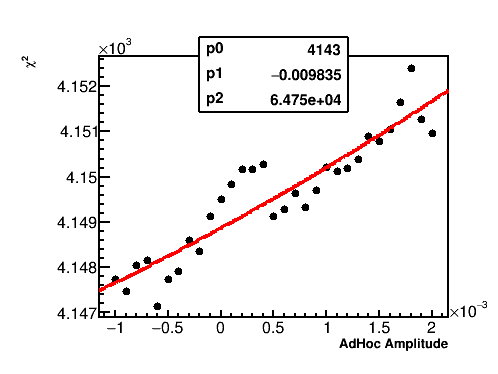
\includegraphics[width=\textwidth]{FullRatio_Chi2_Vs_AdHocAmplitude_Canv}
        \caption{R-Method \chisq versus pileup multiplier. The parabolic fit equation used was $y = p_{2}(x - p_{1})^{2} + p_{0}.$}
    \end{subfigure}% %you need this % here to add spacing between subfigures
    \hspace{1cm}
    \begin{subfigure}[t]{0.45\textwidth}
        \centering
        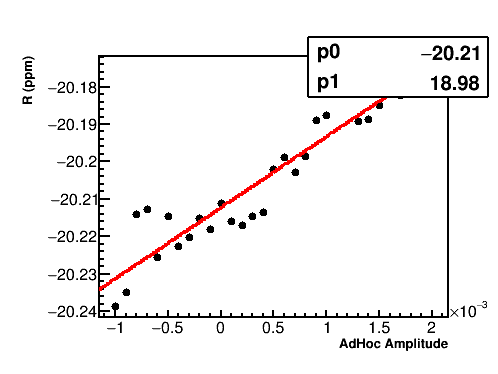
\includegraphics[width=\textwidth]{FullRatio_R_Vs_AdHocAmplitude_Canv}
        \caption{R-Method $R$ versus pileup multiplier. The parameter $p_{1}$ gives the sensitivity of $R$ to the value of the pileup multiplier, with units in ppm.}
    \end{subfigure}
\caption[]{Fix all captions. Data are from the 60h dataset.}
\label{fig:AdHocGainScan}
\end{figure}





\begin{landscape}
\begin{figure}[h]
\centering
    \begin{subfigure}[t]{0.4\textwidth}
        \centering
        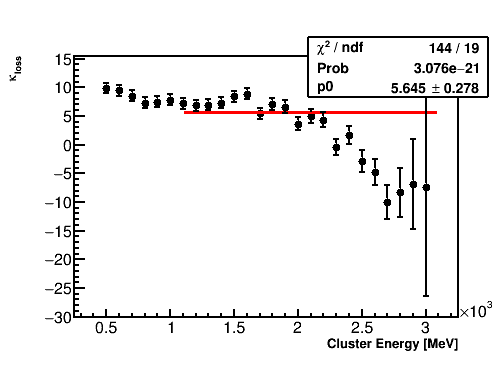
\includegraphics[width=\textwidth]{TMethod_kappa_loss_Vs_EBin_Canv_HK-0}
        \caption{}
    \end{subfigure}% %you need this % here to add spacing between subfigures
    \hspace{1cm}
    \begin{subfigure}[t]{0.4\textwidth}
        \centering
        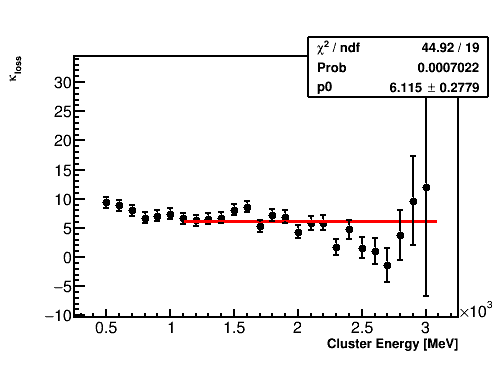
\includegraphics[width=\textwidth]{TMethod_kappa_loss_Vs_EBin_Canv_HK-5p1}
        \caption{}
    \end{subfigure}
    \hspace{1cm}
    \begin{subfigure}[t]{0.4\textwidth}
        \centering
        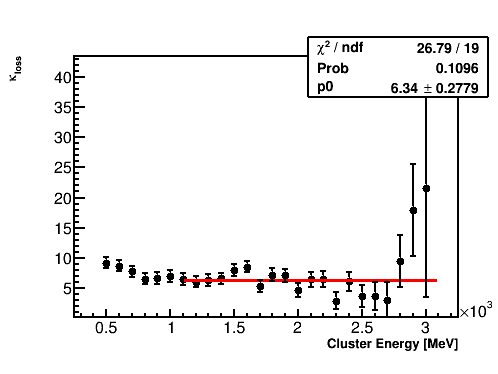
\includegraphics[width=\textwidth]{TMethod_kappa_loss_Vs_EBin_Canv_HK-7p5}
        \caption{}
    \end{subfigure}

    \begin{subfigure}[t]{0.4\textwidth}
        \centering
        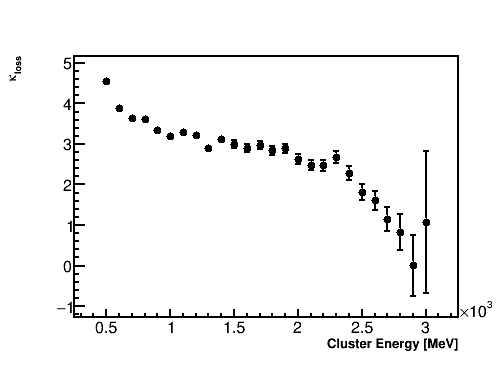
\includegraphics[width=\textwidth]{TMethod_kappa_loss_Vs_EBin_Canv_EG-0}
        \caption{}
    \end{subfigure}% %you need this % here to add spacing between subfigures
    \hspace{1cm}
    \begin{subfigure}[t]{0.4\textwidth}
        \centering
        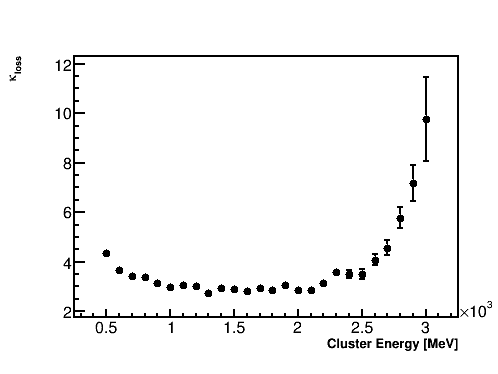
\includegraphics[width=\textwidth]{TMethod_kappa_loss_Vs_EBin_Canv_EG-11p2}
        \caption{}
    \end{subfigure}
    \hspace{1cm}
    \begin{subfigure}[t]{0.4\textwidth}
        \centering
        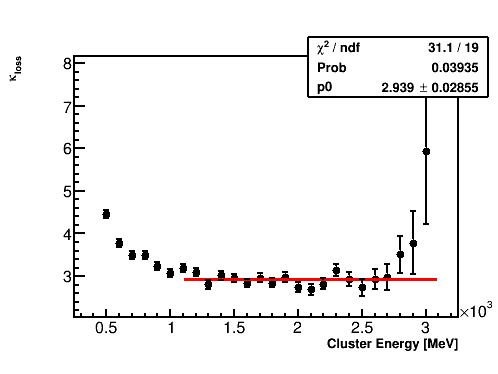
\includegraphics[width=\textwidth]{TMethod_kappa_loss_Vs_EBin_Canv_EG-6p0}
        \caption{}
    \end{subfigure}
\caption[]{}
\label{fig:EBinKloss}
\end{figure}
\end{landscape}





\begin{table}[h]
\centering
% \setlength\tabcolsep{10pt}
\renewcommand{\arraystretch}{1.2}
\begin{tabularx}{0.9\linewidth}{XHGHG}
  \hline
    \multicolumn{5}{c}{\textbf{Residual Gain Tests}} \\
  \hline\hline
            & \multicolumn{2}{c}{$\chi^{2}_{min}$} & \multicolumn{2}{c}{flat $\kappa_{loss}$} \\
  \cmidrule(lr){2-3}\cmidrule(lr){4-5}
    Dataset & \multicolumn{1}{c}{$A_{g} \times 10^{-4}$} & \multicolumn{1}{c}{p value} & \multicolumn{1}{c}{$A_{g} \times 10^{-4}$} & \multicolumn{1}{c}{p value} \\
  \hline
    60h & 8.5 & 0.81 & 8.5 & 0.81 \\
    HighKick & 5.1 & \sim 0 & 7.5 & 0.11 \\
    9d & 8.4 & 0.17 & 10.0 & 0.25 \\
    Endgame & 11.2 & \sim 0 & 6.0 & 0.04 \\
  \hline
\end{tabularx}
\caption[]{}
\label{tab:AdHocGainTests}
\end{table}


\begin{table}[h]
\centering
% \setlength\tabcolsep{10pt}
\renewcommand{\arraystretch}{1.2}
\begin{tabularx}{0.9\linewidth}{XOOJ}
  \hline
    \multicolumn{4}{c}{\textbf{Systematic Error Due to Residual Gain}} \\
  \hline\hline
    Dataset & \thead{Fit Method} & \multicolumn{1}{c}{$ \chi^{2}_{min} \quad \delta R$} & \multicolumn{1}{c}{flat $\kappa_{loss}$ $\boldsymbol{\delta R}$}  \\
  \hline
    \multirow{2}{*}{60h} & T & 28.7 & 28.7 \\
                         & R & 22.9 & 22.9 \\
  \hline
    \multirow{2}{*}{HighKick} & T & 1.0 & 11.8 \\
                              & R & 1.8 & 15.3 \\
  \hline
    \multirow{2}{*}{9d} & T & 18.1 & 24.4 \\
                        & R & 15.2 & 19.1 \\
  \hline
    \multirow{2}{*}{Endgame} & T & 29.9 & 18.8 \\
                             & R & 8.5 & 6.7 \\
  \hline
\end{tabularx}
\caption[]{}
\label{tab:AdHocGainErr}
\end{table}



